\section{Interaktion durch Raypicking} \label{sec:ar-depth-interaction}

Wie in Kapitel \ref{sec:ar-interaction} beschrieben, bedarf es bei der Umsetzung von Augmented Reality Systemen ein anderes Interaktionsparadigma. Auch wenn die Entwicklung der neuen Tablet und Smartphone Geräte durch Touchscreens eine neue Interaktionsform eingeführt haben, ist sie in den meisten Fällen auf einer zweidimensionalen Ebene beschränkt. In der Entwicklung von Virtual Reality oder voll virtuellen Anwendungen und Spielen wird oft für die Auswahlgeste der Raypicking Mechanismus verwendet, um eine zweidimensionale Interaktion im dreidimensionalen Raum zu ermöglichen. Darüber hinaus gibt es verbesserte semantische Interaktionsformen basierend auf einer zweidimensionalen Toucheingabe, wie von \citet{elmqvist2008semantic} beschrieben.

Hier soll aber zunächst eine Raycasting Variante für Augmented Reality Anwendungen umgesetzt werden, die nicht von einem kompletten Modell in Form von Polygonen oder anderen Primitiven der realen Umgebung ausgeht. Diese AR Interaktion ermöglicht, anhand der Tiefeninformationen, das passende Positionieren von virtuellen Objekten im realen Raum und lässt sich auf weitere Interaktionen erweitern. Voraussetzung für die folgende Umsetzung, ist die entsprechende Kalibrierung und Gleichstellung der intrinsischen Kameraparametern und der Verfügbarkeit der extrinsischen Parameter der realen Kamera. 

\begin{figure}[h]
  \centering
	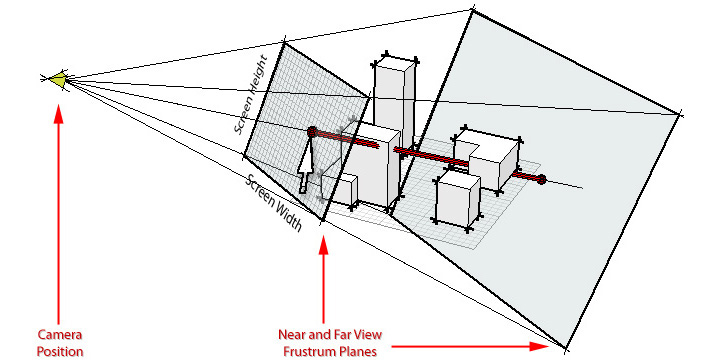
\includegraphics[width=1.0\textwidth]{content/images/methods/interaction.jpg} 
  \caption{Raypicking Visualisierung. Übernommen von \citet{gluUn11:online}}
  \label{fig:interaction}
\end{figure}

Als Erstes wird ein Strahl erzeugt, der durch die Position der virtuellen Kamera und durch den jeweils ausgewählten Punkt auf der Viewingplane läuft. Den Ursprung der virtuellen Kamera bestimmt dabei Google Tangos \enquote{Motion Tracking}. Der gewählte beziehungsweise berührte Punkt auf dem Touchscreen wird dabei zunächst von Pixeln in das Verhältnis \(\left[-1,1\right]\) des Punktes umgerechnet. Hiernach wird die Projektion auf die Viewingplane durch eine Multiplikation mit \(T\) aus Gleichung \ref{eq:unprojection} rückgängig gemacht. Die Gerade aus den beiden Punkten kann danach genutzt werden, um den Schnitt von Objekten vor der Kamera zu ermitteln. \citep{OpenG86:online} 

\begin{equation} \label{eq:unprojection}
T  = MV_{ModelView}^{-1} * P_{Projection}^{-1}
\end{equation}

Angewendet auf die Tiefeninformation aus Tangos \enquote{Depth Perception} wird die Punktewolke, wie in Abbildung \ref{fig:interaction} anstelle der Objekte, vor die Kamera projiziert. In den projizierten Punkten wird danach der entsprechende Punkt gesucht, welcher sich am nächsten am zuvor bestimmten Strahl befindet. Durch diese beschriebenen Schritte kann der Nutzer mit einer zweidimensionalen Geste einen Punkt in der Tiefe bestimmen. Diese Methode kann zudem um die Ermittlung einer Ebenennormalen erweitert werden. Hierzu werden um den selektierten Punkte Nachbarn gefunden, mit denen durch RANSAC eine Ebene ermittelt wird. Durch die ermittelte Ebenennormale können virtuelle Objekte dann nicht nur an die ausgewählte Stelle positioniert werden, sondern auch an der realen Oberflächenausrichtung ausgerichtet werden.

